\documentclass[a4paper, adobefonts]{ctexart}

\usepackage[top=1.2in, bottom=1.2in, left=1in, right=1in]{geometry}
\usepackage{minted, graphicx, hyperref}

\hypersetup{colorlinks=true, linkcolor=blue}

\title{操作系统实验报告8}
\author{蔡日骏\quad12348003}

\begin{document}
\maketitle

\section{简介}
本次实验中对AssignmentOS进行扩展,添加了对信号量的支持。具体来说,是在内核中
实现了对\verb|sem_init|、\verb|sem_p|、\verb|sem_v|三个系统调用的支持。此外,
为了方便测试,本次内核中也加入了对信号处理的支持,目前只实现了\verb|SIGINT|
信号。

\section{实现}
信号量的实现比较简单。由于AssignmentOS只支持单处理器,因此通过禁用中断方式实现
会更方便。

由于信号量需要在内核态内存中处理,但内核态内存容量有限,因此需要及时回收使用完成
的信号量,另外,信号量还需要被多个进程共享,因此需要对信号量进行引用计数,同时
在进程控制数据结构中记录该进程持有的信号量。

在进程\verb|fork|的时候,需要增加进程目前持有的信号量的引用计数。进程结束时,
需要减少进程目前持有的信号量的引用计数。实现如下:

\begin{minted}{c}
/* _sys_fork() */
for(i = 0; i < t->sem_list_size; ++i)
    ++t->sem_list[i]->rc;

/* sys_exit */
for(i = 0; i < CURRENT_TASK->sem_list_size; ++i)
    --CURRENT_TASK->sem_list[i]->rc;
\end{minted}

在信号量的实现上,定义了以下的数据类型:

\begin{minted}{c}
/* 内核态中 */
struct sem_val_t
{
    int val;    /* 信号量当前值 */
    int rc;     /* 信号量引用计数 */
};
typedef struct sem_val_t *_sem_t;

/* 用户态中 */
typedef void *sem_t;    /* 对应内核中的_sem_t */
\end{minted}

\subsection{sem\_*的实现}
\verb|sem_*|系统调用的原型如下:

\begin{minted}{c}
bool sem_init(sem_t *s, int val);   /* 把s指向的信号量初始化成val */
void sem_p(sem_t s);                /* 信号量P操作 */
void sem_v(sem_t s);                /* 信号量V操作 */
\end{minted}

\verb|sem_init|系统调用的工作是查找空闲的信号量SLOT,并对其值进行初始化。

\begin{minted}{c}
int sys_sem_init(int s, int val, int _p3)
{
    if(CURRENT_TASK->sem_list_size == SEM_PER_PROCESS)
    return false;               /* 已达到进程允许拥有的信号量数量 */
    size_t i;
    for(i = 0; i < SEMAPHORE_NUM; ++i) {
        if(SEMAPHORES[i].rc == 0) {
            ++SEMAPHORES[i].rc;             /* 增加信号量引用计数 */
            SEMAPHORES[i].val = val;        /* 初始化信号量值 */
            *(_sem_t *)s = &SEMAPHORES[i];
            CURRENT_TASK->
                sem_list[CURRENT_TASK->sem_list_size++] = *(_sem_t *)s;
            return true;
        }
    }
}
\end{minted}

\verb|sem_p|和\verb|sem_v|系统调用的实现比较简单:

\begin{minted}{c}
int sys_sem_p(int _s, int _p2, int _p3)
{
    cli();                          /* 关闭中断处理 */
    _sem_t s = (_sem_t)_s;
    while(s->val <= 0)
        wait_event(WAIT_SEMAPHORE); /* 挂起当前进程,进行任务调度 */
    --s->val;                       /* 减少信号量的值 */
    sti();                          /* 打开中断处理 */
}

int sys_sem_v(int _s, int _p2, int _p3)
{
    cli();                          /* 关闭中断处理 */
    _sem_t s = (_sem_t)_s;
    ++s->val;                       /* 增加信号量的值 */
    wake_up_event(WAIT_SEMAPHORE);  /* 尝试唤醒被阻塞的进程 */
    sti();                          /* 打开中断处理 */
}
\end{minted}

\subsection{SIGINT信号处理实现}
\verb|SIGINT|信号为当用户按下Ctrl+C组合键时,内核向当前前台进程发送的一个信号。
在默认情况下,进程接收到该进程时会通过\verb|sys_exit|函数退出自己。

在实现上,需要在\verb|0x21|号中断处理函数处理完IRQ1后检查键盘缓冲区队列堆头的
键盘扫描码,如果用户按下的是Ctrl+C,则调用当前前台进程的信号处理函数。

注意该信号只对前台进程起作用,后台进程无法接收到该信号。

\begin{minted}{c}
if(front_kbbuf(&KBBUF) == 0x12e &&      /* 0x1为Ctrl,0x2e为C */
    FOREGROUND_TASK && FOREGROUND_TASK->sigint_handler) {
    /* SIGINT */
    pop_kbbuf(&KBBUF);
    FOREGROUND_TASK->sigint_handler();
}
\end{minted}

\section{演示}
在终端中运行\verb|sem|启动信号量测试程序。

该程序演示了信号量实现生产者——消费者模型。程序启动后会通过\verb|fork|系统调用
成3个子进程,随后父进程成为生产者,每个子进程都是一个消费者。

\begin{minted}{c}
void semaphore_test()
{
    /* buf_size和后面的BUF数组在共享内存中 */
    buf_size = 0;
    char str_buf[16];
    uint8_t child_color;

    /* 初始化信号量 */
    sem_t buf_s, empty_s, full_s;
    sem_init(&buf_s, 1);
    sem_init(&empty_s, 0);
    sem_init(&full_s, 10);

    /* Fork出3个子进程,每个进程使用不同颜色输出 */
    if((child_color = 0xF1, fork()) &&
       (child_color = 0x6A, fork()) &&
       (child_color = 0x3C, fork())) {
        /* 父进程,生产者 */
        unsigned int n = CLOCK;
        while(true) {
            sem_p(full_s);

            n = rng(n);
            itos(n % 1000, str_buf);
            print_str("Producer: producing, it will take ", 0x07);
            print_str(str_buf, 0x07);
            print_str(" ms.\n", 0x07);
            sleep(n % 1000);
            sem_p(buf_s);
            BUF[buf_size++] = n;
            sem_v(buf_s);
            print_str("Producer: finished.\n", 0x07);

            sem_v(empty_s);
        }
    } else {
        /* 子进程,消费者 */
        unsigned int n;
        while(true) {
            sem_p(empty_s);

            sem_p(buf_s);
            n = BUF[--buf_size] % 3219;
            sem_v(buf_s);

            sem_v(full_s);

            itos(n, str_buf);
            print_str("Consumer: got, consuming, it will take ", child_color);
            print_str(str_buf, child_color);
            print_str(" ms.\n", child_color);
            sleep(n);
            print_str("Consumer: finished.\n", child_color);
        }
    }
}
\end{minted}

效果如图。生产者输出为黑底灰字,消费者输出为彩色,不同消费者输出颜色不同。
\emph{由于IO操作不是线程安全的,在某些模拟器下可能会偶尔出现输出错位的情况。}

\begin{figure}[htp!]
    \center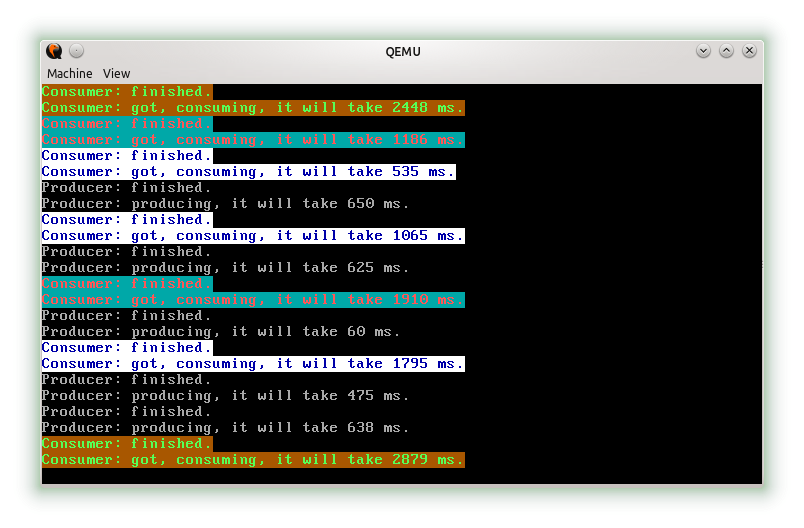
\includegraphics[scale=0.75]{sem.png}
\end{figure}

\end{document}
